\documentclass[11pt,a4paper]{article}

% Journal-neutral, self-contained manuscript: no publisher class or external artwork.
\usepackage[a4paper,margin=27mm,headheight=14pt]{geometry}
\usepackage[T1]{fontenc}
\usepackage[utf8]{inputenc}
\usepackage{newtxtext}
\usepackage{microtype}
\usepackage{amsmath,amsthm,mathtools}
\usepackage{newtxmath}
\usepackage{booktabs,tabularx,array}
\usepackage{graphicx}
\usepackage{float}
\usepackage{pgfplots}
\usepackage[hidelinks]{hyperref}
\usepackage[font=small,labelfont=bf,labelsep=period]{caption}
\pgfplotsset{compat=1.18}
\hypersetup{pdftitle={Pregeometric Relational Dynamics and Universal Causal Structure},pdfauthor={Andrei Preece and Boris Batenin},pdfsubject={Permutation-invariant graph phase selection and effective causal order}}
\setlength{\parindent}{1.2em}
\setlength{\parskip}{0pt}
\setlength{\textfloatsep}{14pt plus 2pt minus 3pt}
\setlength{\intextsep}{12pt plus 2pt minus 2pt}
\setlength{\abovedisplayskip}{9pt plus 2pt minus 3pt}
\setlength{\belowdisplayskip}{9pt plus 2pt minus 3pt}
\emergencystretch=1.5em
\numberwithin{equation}{section}
\newtheorem{theorem}{Theorem}[section]
\newtheorem{proposition}[theorem]{Proposition}
\newtheorem{nogo}[theorem]{No-go statement}
\newcommand{\G}{\mathcal{G}}
\newcommand{\EN}{E_N}
\newcommand{\CN}{C_N}
\newcommand{\barb}{\bar b}
\newcommand{\norm}[1]{\left\lVert#1\right\rVert}
\newcommand{\dd}{\mathrm d}
\newcommand{\1}{\mathbf{1}}
\newcommand{\tr}{\operatorname{tr}}
\newcommand{\dist}{\operatorname{d}}
\newcommand{\TV}{\operatorname{TV}}
\newcommand{\arcosh}{\operatorname{arcosh}}
\newcommand{\st}{\mathrel{\sim}}
\newcolumntype{Y}{>{\raggedright\arraybackslash}X}

\title{\bfseries\Large Pregeometric Relational Dynamics and Universal Causal Structure\\[0.55em]
\normalfont\large A Permutation-Invariant Phase-Selection Witness:\\
Quasilocality, Cone Locking, and the Boundary of Temporal Orientation}
\author{Andrei Preece \quad and \quad Boris Batenin\\[0.45em]
\normalsize Independent Researchers, Berlin, Germany}
\date{12 October 2026}
\begin{document}
\maketitle
\vspace{-1.7em}
\begin{abstract}
\noindent
We give a finite, explicitly defined, permutation-invariant stochastic relational model in which a one-dimensional quasilocal graph phase is selected with a quantitative equilibrium probability bound. The ground states are precisely unembedded cycles; their rescaled intrinsic metric-measure spaces converge to a circle, with no preferred labelling, spatial orientation, or embedding. An independent orthogonally equivariant relaxation of a positive multicomponent stiffness matrix suppresses relative propagation-speed defects exponentially. Once graph equilibration and stiffness relaxation have taken place, the selected cycles remain metastable over any fixed observational time window with probability tending to one. Their normalised retarded wave responses converge to a common one-dimensional continuum causal propagator, and finite-system response tails disappear uniformly outside buffered cones. We distinguish the derived effective forward cone from the origin of the time arrow: the latter is not obtained from an undirected graph or from a reversible equilibrium state; forward Markov evolution, a non-equilibrium preparation and retarded initial data remain explicit inputs. This is a constructive existence result in a deliberately restricted toy class---not a derivation of $3+1$-dimensional spacetime, a closed Hamiltonian attractor, gauge fields, or the observed laws of gravity.
\end{abstract}
\noindent\textbf{Keywords:}\enspace emergent quasilocality; permutation invariance; Gibbs graph dynamics; metastability; common cone; response tails; reconstruction; time reversal.

\section{Scope and relation to previous work}
This paper uses five established ingredients from the companion analysis~\cite{companion} without repeating their detailed derivations (see also the preceding unified preprint~\cite{original}): (i) an undirected relation is not itself a response or a Lorentzian causal order; (ii) a finite connected graph generally has analytic, nonzero off-site response tails; (iii) a common cone on the retained massless sector requires a scalar leading stiffness operator, or a mechanism making its trace-free part small; (iv) a continuum Green density is the response matrix divided by the vertex measure; and (v) on prescribed cycles, wave responses converge and buffered exterior tails vanish under controlled refinement. The Maxwell control sector of the companion manuscript is not needed to prove the statements below and is deliberately omitted.

\noindent\textit{Terminology.} ``Theorem'' means proved for the finite models and limits explicitly specified here. ``Conditional interpretation'' denotes an identification requiring an effective clock, metric, and state preparation. ``Open'' denotes a physical step not shown by this construction.

\section{A neutral, label-free relational dynamics}
\subsection{Graph state and energy}
Fix $N\geq5$. Let $\G_N$ be the finite set of all simple undirected graphs on vertex set $\{1,\ldots,N\}$. The vertices are bookkeeping labels: no point, distance, coordinate, preferred cycle, orientation, or manifold is assigned. For $A\in\G_N$, write $\deg_A(i)$ for a degree and $k(A)$ for the number of connected components, with isolated vertices counted.
\begin{equation}\label{eq:energy}
 E_N(A)=\sum_{i=1}^{N}\bigl(\deg_A(i)-2\bigr)^2+\bigl(k(A)-1\bigr).
\end{equation}
$E_N$ is a nonnegative integer and is invariant under every permutation of vertex labels. Its exact valence-two preference and global connectivity penalty are microscopic choices of the model, not consequences of a structure-free relational axiom. This is a crucial restriction on the meaning of emergence.

\subsection{Autonomous edge-flip dynamics}
Put $M_N=N(N-1)/2$. Two graphs are neighbours when a single unordered edge is toggled. At fixed inverse graph temperature $\beta>0$, use the continuous-time Markov generator $Q_N$ with the rates
\begin{align}
 q_\beta(A,A')&=M_N^{-1}\min\bigl\{1,\exp[-\beta(E_N(A')-E_N(A))]\bigr\}
 &&(A\sim A'),\label{eq:rates}\\[-2pt]
 q_\beta(A,A)&=-\sum_{A'\neq A}q_\beta(A,A').\nonumber
\end{align}
This law acts only on undirected relation matrices, is equivariant under all vertex permutations, and is well-defined without embedding. It does, however, specify a forward Markov semigroup; temporal reversibility and the effective thermodynamic arrow are discussed separately in Section~\ref{sec:arrow}; see also standard background on finite Markov chains~\cite{markov}.

\section{Selection and metastability of a cycle phase}
\begin{theorem}[Exact minima, concentration, and persistence]\label{thm:cycle}
For $N\geq5$ and the energy and rates in \eqref{eq:energy}--\eqref{eq:rates}:
\begin{enumerate}
\item[(a)] $E_N(A)=0$ precisely for connected $N$-cycles. Their number on the labelled vertex set is $K_N=(N-1)!/2$. All these configurations are equivalent under relabelling; no one embedded cycle is singled out.
\item[(b)] The chain is irreducible and has unique stationary law $\pi_{N,\beta}(A)=Z_{N,\beta}^{-1}\exp[-\beta E_N(A)]$. Moreover,
\begin{equation}\label{eq:concentration}
 \pi_{N,\beta}(\text{non-cycle})\leq\frac{2^{M_N}}{K_N}\,e^{-\beta}.
\end{equation}
\item[(c)] Starting from any exact cycle, the probability of at least one graph change during a time window $[0,T]$ is at most $Te^{-2\beta}$.
\item[(d)] If an additional permutation-invariant energy $V_N$ satisfies $\sup_A|V_N(A)|\leq\eta<1/2$, all global minima of $E_N+V_N$ remain among the cycles, and its Gibbs law satisfies
\begin{equation}\label{eq:robust}
 \pi'_{N,\beta}(\text{non-cycle})\leq\frac{2^{M_N}}{K_N}\,e^{-\beta(1-2\eta)}.
\end{equation}
\end{enumerate}
\end{theorem}
\begin{proof}
Since each term in \eqref{eq:energy} is nonnegative, $E_N=0$ forces all degrees to be two and $k=1$. A finite connected simple $2$-regular graph is exactly one cycle traversing all $N$ vertices. Conversely, such a cycle has $E_N=0$. The number of undirected labelled cycles equals $N!/(2N)=K_N$. Every graph can be reached from any other by finitely many toggles; all rates in \eqref{eq:rates} are strictly positive, giving irreducibility. Detailed balance holds because
$e^{-\beta E(A)}q(A,A')=e^{-\beta E(A')}q(A',A)$.
Thus the Gibbs distribution is unique. Each non-minimum has integer $E_N\geq1$. Comparing the total non-cycle Gibbs weight with the $K_N$ cycle weights gives \eqref{eq:concentration}. Any single-edge toggle starting from a cycle creates precisely two vertices of degree $1$ (deletion) or two vertices of degree $3$ (chord addition), while leaving the component count one. Its energy is therefore exactly $2$. As the total proposal rate equals one, the exit rate of each cycle is $e^{-2\beta}$, so the exponential holding-time estimate gives (c). Finally, a cycle has perturbed energy at most $\eta$ while any non-cycle has energy at least $1-\eta$. The ratio of their Gibbs weights is bounded by $e^{-\beta(1-2\eta)}$, proving (d).
\end{proof}
\noindent\textit{Explicit asymptotic parameter choice.} Set $\beta_N=M_N\log2+N$. Then $\pi_{N,\beta_N}(\text{non-cycle})\leq e^{-N}/K_N\leq e^{-N}$, and the departure probability in a fixed $T$-window is at most $Te^{-2\beta_N}$. These bounds are intentionally conservative; they establish a limit and make no efficient-mixing claim.

For each finite $N$, irreducibility gives convergence from arbitrary initial graph laws to $\pi_{N,\beta_N}$ as time $\tau\to\infty$. Choose a preparation time $\tau_N$ so that the total variation distance from equilibrium is at most $e^{-N}$. Such times exist but may be extremely long; uniform or polynomial mixing time is \emph{not} proved. At the observation time $\tau_N$, the probability of not being a cycle is at most $2e^{-N}$.

\section{An intrinsic metric-measure continuum}
\begin{theorem}[Intrinsic circle limit]\label{thm:circle}
Conditioned on selection of any ground-state graph $C_N$, endow its vertices with shortest-path distance $d_N(i,j)=a_Nd_{C_N}(i,j)$, where $a_N=\ell/N$ for fixed $\ell>0$, and with vertex measure $\mu_N(\{i\})=1/N$. Then the metric-measure cycle converges to the length-$\ell$ circle $S^1_\ell$ with uniform measure in the Gromov--Hausdorff--Prokhorov sense; a distance bound of $a_N/2$ suffices. The limit is independent of all labellings and of the two orientations of a cycle.
\end{theorem}
\begin{proof}
Choose any graph isomorphism from $C_N$ to a regular $N$-gon on an abstract length-$\ell$ circle. This is an identification for the proof, not a microscopic embedding or physically preferred coordinate chart. The intrinsic scaled graph distance agrees with the shorter arc length between sampled circle points. Every point of the circle is within arc distance $a_N/2$ of a sampled vertex, proving the asserted Hausdorff bound in this common metric. Couple uniform circle measure to uniform vertex measure by sending each equal-length Voronoi cell to its central vertex; the transport distance is at most $a_N/2$. The corresponding Prokhorov bound follows. Any other isomorphism differs by a dihedral symmetry and yields the same metric-measure isomorphism class.
\end{proof}
This is one spatial dimension only. The choice of valence $2$ is precisely why a one-dimensional result is possible; neither an emergent three-dimensional phase nor a Lorentzian signature is implied by Theorem~\ref{thm:circle}.

\section{Multicomponent cone locking by an invariant law}
\subsection{Isotropisation of stiffness}
At each graph vertex take a real $r$-component field $q_i$, with $r\geq2$, and an initially arbitrary positive-definite symmetric component matrix $B_0$. Let $B(s)$ be an autonomous additional effective degree of freedom governed by the $O(r)$-equivariant law
\begin{equation}\label{eq:relax}
 \frac{\dd B}{\dd s}=-\gamma\left[B-\frac{\tr B}{r}I_r\right],
 \qquad\gamma>0,\qquad B(0)=B_0>0.
\end{equation}
The graph and stiffness processes may evolve concurrently. Their use here is dissipative/effective: \eqref{eq:relax} is not generated by the closed Hamiltonian discussed in the companion analysis and is not passed off as a Hamiltonian attractor.
\begin{theorem}[Global scalarisation]\label{thm:scalar}
Writing $\barb=\tr(B_0)/r$, for all $s\geq0$,
\begin{equation}\label{eq:scalar}
\begin{aligned}
 B(s)&=\barb I_r+e^{-\gamma s}(B_0-\barb I_r),\\
 \norm{B(s)-\barb I_r}&=e^{-\gamma s}\norm{B_0-\barb I_r}.
\end{aligned}
\end{equation}
$B(s)$ remains positive definite. Its eigenvalue-dependent leading propagation speeds $v_a(s)=\sqrt{\lambda_a(B(s))}$ converge exponentially to the single speed $v=\sqrt{\barb}$. In particular,
\begin{equation}\label{eq:speeds}
 \max_a|v_a(s)-\sqrt{\barb}|\leq
 \frac{e^{-\gamma s}}{\sqrt{\barb}}\norm{B_0-\barb I_r}.
\end{equation}
\end{theorem}
\begin{proof}
Taking the trace in \eqref{eq:relax} shows $\tr B(s)=\tr B_0$. The trace-free part obeys a scalar linear ODE with decay rate $\gamma$, giving \eqref{eq:scalar}. Its solution is a convex combination of $B_0$ and $\barb I$ and is therefore positive. The eigenvalues evolve as $\barb+e^{-\gamma s}(\lambda_a(B_0)-\barb)$. The identity $|\sqrt{x}-\sqrt{y}|=|x-y|/(\sqrt{x}+\sqrt{y})$ gives \eqref{eq:speeds}. Orthogonal conjugation commutes with both trace and the right-hand side of \eqref{eq:relax}, proving $O(r)$-equivariance.
\end{proof}
The law \eqref{eq:relax} builds in a scalarising mechanism through its trace-free damping; it is not a spontaneous consequence of graph rearrangement. Unlike fixing equal speeds by fiat, however, it admits arbitrary initially unequal positive sector stiffnesses and gives an exact attraction rate. A closed-system microscopic realisation of this dissipative evolution remains open.

\subsection{Coupled wave test on the selected graph}
For a selected cycle, define $a_N=\ell/N$ and a field response during the observation window $u\in[0,T]$ by
\begin{equation}\label{eq:wave}
 q''(u)+\left[a_N^{-2}L(C_N)\otimes B(\tau_N+u)\right]q(u)=0,
 \quad q(0)=0,\quad q'(0)=f.
\end{equation}
Here $L(C_N)$ is the unweighted graph Laplacian. The only spatial structure in \eqref{eq:wave} is the graph selected by the permutation-invariant relational process. The factor $a_N^{-2}$ is a subsequent continuum calibration, not an assumed pre-existing distance.
\begin{theorem}[Joint probabilistic cone witness]\label{thm:cone}
Choose $\beta_N=M_N\log2+N$ and times $\tau_N$ large enough that (i) the graph-law total variation distance from $\pi_{N,\beta_N}$ is at most $e^{-N}$, and (ii) $\delta_N/a_N^3\to0$, where $\delta_N=\norm{B_0-\barb I_r}e^{-\gamma\tau_N}$. Then, for every fixed $T>0$, with probability at least
\begin{equation}\label{eq:probability}
 1-2e^{-N}-Te^{-2\beta_N},
\end{equation}
the graph is a cycle at the start of $[\tau_N,\tau_N+T]$ and makes no edge change throughout that window. On this event, after a cycle-to-circle identification the $r$-component velocity-response operators of \eqref{eq:wave} converge strongly and uniformly for $u\in[0,T]$ to those of
\begin{equation}\label{eq:continuum}
 \partial_u^2q(u,x)-\barb\,\partial_x^2q(u,x)=0
 \qquad\text{on }S^1_\ell,
\end{equation}
and their correctly normalised kernels converge uniformly to zero outside every buffered cone $d(x,y)>\sqrt{\barb}\,u+\delta$, $\delta>0$. All $r$ sectors have the same limiting characteristic cone.
\end{theorem}
\begin{proof}[Proof: probability and finite-time stability]
The graph estimate at $\tau_N$ is Theorem~\ref{thm:cycle} plus the total-variation error. Conditional on a cycle, the graph exit rate is $e^{-2\beta_N}$; a union bound gives \eqref{eq:probability}. On this event the graph Laplacian is fixed. Let $K_0=(\barb/a_N^2)L(C_N)\otimes I_r$. The actual time-dependent wave operator is $K_0+E_N(u)$, with operator norm bounded by $m_N=4\delta_N/a_N^2$ since $\norm{L(C_N)}\leq4$. Let $S_0(u)=\sin(u\sqrt{K_0})/\sqrt{K_0}$; the zero-frequency value is $u$, and $\norm{S_0(u)}\leq u$. Duhamel's formula gives
\[
 q(u)=S_0(u)f-\int_0^u S_0(u-s)E_N(s)q(s)\,\dd s.
\]
If $m_NT^2/2<1$, taking suprema and then substituting back yields
\begin{equation}\label{eq:duhamel}
 \sup_{0\leq u\leq T}\norm{U_N(u)-S_0(u)}\leq
 \frac{m_NT^3/2}{1-m_NT^2/2}.
\end{equation}
On a regular cycle, the eigenvalues of $a_N^{-2}L$ on Fourier wave numbers $k$ are $4a_N^{-2}\sin^2(ka_N/2)\to k^2$. Trigonometric-polynomial testing and the bound $\norm{S_0(u)}\leq T$ give uniform strong convergence to the continuum velocity-response operator. By \eqref{eq:duhamel}, the time-dependent response has the same limit. For pointwise kernel control, the discrete Green density is the response matrix divided by the cell mass $a_N$ (not just the unnormalised matrix element). Dividing \eqref{eq:duhamel} by $a_N$ gives an error $O_T(\delta_N/a_N^3)\to0$. For the baseline cycle kernel, the established finite-cycle contour estimate from \cite[Part II]{companion} gives, for $\delta>0$ and $\theta=\arcosh(1+\delta/(vT))$, $v=\sqrt{\barb}$,
\begin{equation}\label{eq:exterior}
\begin{aligned}
 &\sup_{\substack{u\leq T\\d_N(i,j)>vu+\delta}}|G_N^0(u;i,j)|\\
 &\qquad\leq\frac{2T}{a_N\bigl(1-e^{-2\theta\ell/a_N}\bigr)}
 \exp\!\left[-\frac{c(T,\delta)}{a_N}\right],
\end{aligned}
\end{equation}
where $c(T,\delta)=2[\delta\theta-vT(\sinh\theta-\theta)]>0$.
Both terms tend to zero. Finally, the scalar Fourier limit has principal symbol $(-\omega^2+\barb k^2)I_r$, yielding the common characteristic cone.
\end{proof}

\subsection{Why the finite graph still has no strict light cone}
For each fixed selected cycle the velocity-response matrix equals
\[
 S_0(u)=\sum_{m\geq0}\frac{(-1)^m u^{2m+1}K_0^m}{(2m+1)!}.
\]
If $i$ and $j$ have graph distance $d\geq1$, then $(K_0^m)_{ij}=0$ for $m<d$ but $(K_0^d)_{ij}$ has a nonzero shortest-path contribution. Hence its first nonzero Taylor coefficient is proportional to $u^{2d+1}$; the off-site response is not identically zero on any interval $(0,\varepsilon)$. The strictly vanishing exterior emerges only after refinement, measure normalisation, identification, and taking the limit---not at finite $N$.

\section{Operational forward order and the time-arrow obstruction}\label{sec:arrow}
\subsection{An explicit effective oriented partial order}
On the emergent cylinder $\mathbb R\times S^1_\ell$, use the forward time parameter defined by the wave initial-value protocol, and set
\begin{equation}\label{eq:order}
 (t,x)\preceq(s,y)\iff s\geq t\ \text{and}\
 d_{S^1}(x,y)\leq v(s-t),\qquad v=\sqrt{\barb}.
\end{equation}
\begin{proposition}\label{prop:order}
Relation \eqref{eq:order} is a reflexive, transitive, antisymmetric partial order, and the retarded fundamental solution of \eqref{eq:continuum} is supported on its future cones.
\end{proposition}
\begin{proof}
Reflexivity follows from $d(x,x)=0$. Transitivity is the triangle inequality. If events precede each other in both directions, then $s=t$ and distance zero, so they coincide. The one-dimensional d'Alembert formula on the covering line and its periodisation to the circle show that an initially localised velocity disturbance is supported only where $d(x,y)\leq v(s-t)$ for $s\geq t$.
\end{proof}
The word ``oriented'' is valid only relative to the chosen forward evolution parameter and retarded boundary condition. Neither the undirected adjacency matrix nor the selected unmarked cycle contains a preferred direction of time, and neither contains a preferred clockwise orientation.

\subsection{Nonequilibrium entropy and why it is not an \emph{ex nihilo} time arrow}
For fixed finite $N$, the graph generator $Q_N$ is reversible with respect to $\pi_{N,\beta}$. If $\mu_s$ is an evolving distribution and $h_s(A)=\mu_s(A)/\pi(A)$, then its relative entropy decreases:
\begin{equation}\label{eq:entropy}
\begin{aligned}
 \frac{\dd}{\dd s}D(\mu_s\Vert\pi)
 =-&\frac12\sum_{A,A'}\pi(A)q(A,A')\\[-1pt]
 &\;\times[h_s(A)-h_s(A')]
 [\log h_s(A)-\log h_s(A')]\leq0.
\end{aligned}
\end{equation}
The proof is direct differentiation using detailed balance and the monotonicity of $\log$; it is strictly negative away from equilibrium for positive $\mu_s$ because the graph-flip chain is irreducible. Thus an out-of-equilibrium preparation determines a measurable relaxation direction, while a stationary Gibbs ensemble does not.

\begin{nogo}[Time-reversal symmetric preparation]\label{nogo:time}
Suppose an underlying law and chosen state are invariant under time reversal $\Theta$, and an orientation observable $J$ is odd, $J\circ\Theta=-J$. Then $\langle J\rangle=0$.
\end{nogo}
\begin{proof}
Invariance gives $\langle J\rangle=\langle J\circ\Theta\rangle=-\langle J\rangle$.
\end{proof}
Consequently no nonzero mean time orientation follows from exactly $\Theta$-invariant law and preparation alone. The forward Markov semigroup, trace-free damping \eqref{eq:relax}, and retarded experimental intervention all contain an explicit asymmetric selection. A closed, exactly time-reversal-invariant microscopic system yielding a branchwise internal arrow without imposing such a selection remains the central unsolved step. Accordingly, the combined theorem proves an emergent oriented \emph{effective} causal order under a preparation protocol, not the absolute spontaneous origin of the time direction from neutral relations alone.

\section{Exact finite-size enumeration}
We exhaustively enumerated all $2^{N(N-1)/2}$ undirected graphs for $N=5$ ($1{,}024$ graphs) and $N=6$ ($32{,}768$ graphs), computed energy \eqref{eq:energy}, and evaluated the partition function directly. The number of exact minima agreed with the cycle count $(N-1)!/2$. The results below are deterministic enumeration, not Monte Carlo, and they test only the stated small finite graph model.

At $\beta=4$, the exact equilibrium cycle probabilities are $0.99305256$ ($N=5$) and $0.98458904$ ($N=6$); at $\beta=6$ they rise to $0.99987200$ and $0.99935685$. At $\beta=0$ the corresponding uniform-graph probabilities are $12/1024$ and $60/32768$. These values are obtained by direct finite sums, without stochastic sampling.

\begin{figure}[H]
 \centering
 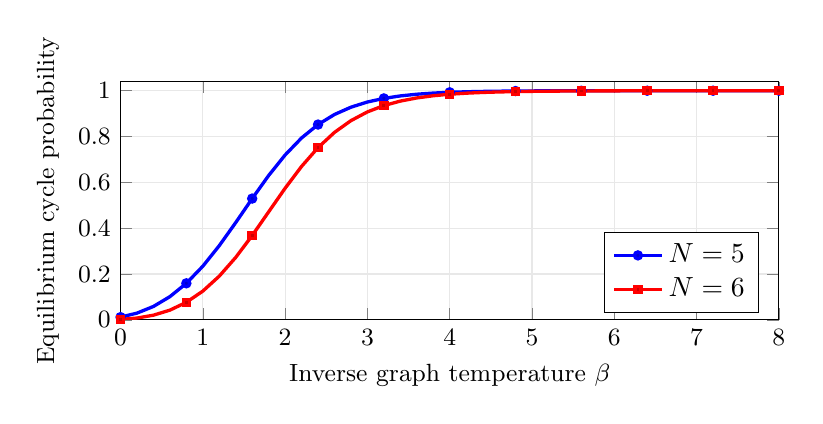
\begin{tikzpicture}
 \begin{axis}[
  width=0.82\linewidth,height=0.38\linewidth,
  xmin=0,xmax=8,ymin=0,ymax=1.04,
  xtick={0,1,2,3,4,5,6,7,8},
  ytick={0,0.2,0.4,0.6,0.8,1},
  xlabel={Inverse graph temperature $\beta$},
  ylabel={Equilibrium cycle probability},
  grid=major,grid style={black!9},
  legend pos=south east,
  every axis plot/.append style={very thick},
  tick label style={font=\small},label style={font=\small}]
 \addplot+[mark=*,mark repeat=4,mark size=1.25pt] coordinates {
(0.00,0.011718750) (0.20,0.029250382) (0.40,0.058361738) (0.60,0.101148753) (0.80,0.159386840) (1.00,0.233977141) (1.20,0.323747423) (1.40,0.424502443) (1.60,0.529236726) (1.80,0.629814525) (2.00,0.719326488) (2.20,0.793760264) (2.40,0.852241887) (2.60,0.896176826) (2.80,0.928085962) (3.00,0.950696804) (3.20,0.966440860) (3.40,0.977270585) (3.60,0.984657671) (3.80,0.989667750) (4.00,0.993052561) (4.20,0.995333382) (4.40,0.996867601) (4.60,0.997898400) (4.80,0.998590424) (5.00,0.999054769) (5.20,0.999366235) (5.40,0.999575106) (5.60,0.999715156) (5.80,0.999809052) (6.00,0.999871999) (6.20,0.999914196) (6.40,0.999942483) (6.60,0.999961445) (6.80,0.999974156) (7.00,0.999982676) (7.20,0.999988387) (7.40,0.999992216) (7.60,0.999994782) (7.80,0.999996502) (8.00,0.999997655)
 };
 \addlegendentry{$N=5$}
 \addplot+[mark=square*,mark repeat=4,mark size=1.1pt] coordinates {
(0.00,0.001831055) (0.20,0.007674247) (0.40,0.020258106) (0.60,0.042265821) (0.80,0.076415583) (1.00,0.125280575) (1.20,0.190646231) (1.40,0.272487091) (1.60,0.367965438) (1.80,0.471182607) (2.00,0.574270613) (2.20,0.669548727) (2.40,0.751579647) (2.60,0.818047995) (2.80,0.869340121) (3.00,0.907474175) (3.20,0.935067429) (3.40,0.954660344) (3.60,0.968400023) (3.80,0.977961673) (4.00,0.984589037) (4.20,0.989176708) (4.40,0.992355133) (4.60,0.994562851) (4.80,0.996102458) (5.00,0.997181777) (5.20,0.997943226) (5.40,0.998484361) (5.60,0.998872077) (5.80,0.999152343) (6.00,0.999356851) (6.20,0.999507541) (6.40,0.999619681) (6.60,0.999703957) (6.80,0.999767904) (7.00,0.999816870) (7.20,0.999854687) (7.40,0.999884126) (7.60,0.999907208) (7.80,0.999925421) (8.00,0.999939873)
 };
 \addlegendentry{$N=6$}
 \end{axis}
 \end{tikzpicture}
 \caption{Exact Gibbs probabilities for the unembedded cycle phase. Increasing $\beta$ is part of the specified dynamical model; $N=5,6$ provide no evidence for a large-$N$ mixing rate.}\label{fig:phase}
\end{figure}

\begin{figure}[H]
 \centering
 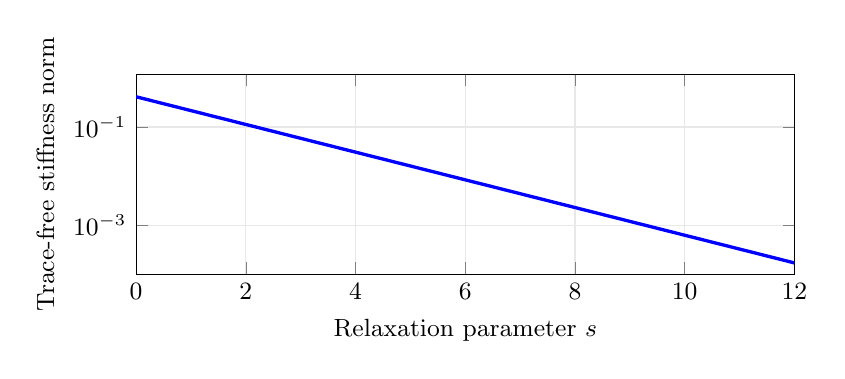
\begin{tikzpicture}
 \begin{semilogyaxis}[
  width=0.82\linewidth,height=0.34\linewidth,
  xmin=0,xmax=12,ymin=1e-4,ymax=1.2,
  xtick={0,2,4,6,8,10,12},
  xlabel={Relaxation parameter $s$},
  ylabel={Trace-free stiffness norm},
  grid=major,grid style={black!9},
  tick label style={font=\small},label style={font=\small}]
  \addplot+[no marks,very thick,domain=0:12,samples=80] {(1.44-(0.64+1+1.44)/3)*exp(-0.65*x)};
 \end{semilogyaxis}
 \end{tikzpicture}
 \caption{Exact trace-free stiffness decay for $B_0=\operatorname{diag}(0.64,1,1.44)$ and $\gamma=0.65$. The result follows analytically from the assumed isotropisation law; it is not a measured fundamental interaction.}\label{fig:relaxation}
\end{figure}
The enumeration and associated figure data are generated from the specified finite model. The numerical values are cross-checks of Theorem~\ref{thm:cycle} and \eqref{eq:scalar}, not independent proof of emergence of a physical universe.

\section{Falsification criteria and open problems}
\begin{table}[H]
\caption{Demonstrated results and limitations of their transfer to physical spacetime.}\label{tab:falsification}
\small
\renewcommand{\arraystretch}{1.2}
\setlength{\tabcolsep}{5pt}
\begin{tabularx}{\linewidth}{@{}p{0.23\linewidth}YY@{}}
\toprule
Required interface & Demonstrated in this model & Potential failure of a physical transfer \\
\midrule
Neutral graph $\to$ local sector & Exact selection of unembedded one-dimensional cycles for the specified $E_N$ & Absence of a stable low-dimensional phase for physically motivated, non-tailored energy laws \\
\addlinespace[2pt]
Local sector $\to$ continuum geometry & Metric-measure convergence for $C_N$; calibration $\ell/N$ supplied & No scale-independent spatial metric, stable measure, or dimensional plateau \\
\addlinespace[2pt]
Several modes $\to$ common cone & Explicit exponential attraction of $B(s)$ to scalar form & Radiative instability, sector-dependent couplings, or symmetry-breaking noise \\
\addlinespace[2pt]
Finite response $\to$ limiting cone & Strong response and exterior-kernel bounds on prepared cycle phases & Failure under typical dynamic backgrounds, perturbations, or internal-state probes \\
\addlinespace[2pt]
Cone $\to$ oriented causal order & Partial order given an effective forward clock and retarded data & No internally selectable arrow, or only a coordinate convention \\
\addlinespace[2pt]
Toy phase $\to$ physical spacetime & \emph{Not established} & No three-dimensional phase, Lorentzian field content, quantum stability, or gravitational dynamics \\
\bottomrule
\end{tabularx}
\end{table}

\subsection{The closed-system bridge still to be established}
The next theorem should not merely substitute a three-dimensional target graph into $E_N$ or decree scalar stiffness by a penalty. A persuasive next result must exhibit one label-invariant \emph{closed} microscopic dynamics, a large basin of unbiased initial data, and a physically justified scaling regime in which: (i) the effective dimension is selected rather than programmed; (ii) a quasilocal measure and reconstruction are stable under perturbations; (iii) multiple observable sectors flow to a common principal cone without imposed common kinetic coefficients; (iv) an internal record/clock selects orientation without an external forward arrow; and (v) correlations, responses, and nonlinear/quantum observables obey the correct continuum tests. None of these five conditions is proved here in the unrestricted setting.

\subsection{Related mathematical methods and their limits}
For future investigations, the OpenAI Math repository~\cite{openai_math,openai_catalog} includes work on random planar-map metric-measure and spectral scaling (family 211), graph-metric embeddings (family 089), graph switch-chain mixing (family 131), and relabelling-invariant graph thresholds (family 186). These are potentially useful method families, but their hypotheses differ from the specific energy, generator, and Lorentzian wave evolution here. In particular, graph switch-chain mixing at fixed degree cannot be substituted for a mixing-time proof of our single-edge Metropolis chain, and convergence to a random-surface metric does not imply causal signature. The repository itself warns that not all posted results are formally verified and that some could contain errors. No such result is used as an unproved black box in Theorems~\ref{thm:cycle}--\ref{nogo:time}.

\section{Conclusion}
The existence claim established here is narrow but mathematical: one fully specified symmetric graph evolution can select a stable quasilocal phase from unlabeled neutral connectivity; one explicit equivariant relaxation can remove initially unequal wave-sector stiffnesses; and, under a controlled preparation and scaling limit, a common retarded characteristic cone yields an effective oriented partial order. The chain is quantified by finite-$N$ Gibbs and exit bounds, metric-measure convergence, stiffness-decay estimates, and normalised Green-kernel control. The decisive unresolved issue is structural, not terminological: the arrow of time, dimension, and universality mechanisms were partly encoded in the update law or effective sector, and were not derived from an autonomous closed, reversible, and truly geometry-neutral microscopic physics. The present result should therefore be read as an explicit benchmark that future non-programmed emergence mechanisms must equal or improve---not as a completion of the full pregeometric programme.

\begin{thebibliography}{9}
\bibitem{companion}
A.~Preece and B.~Batenin, \emph{Pregeometric Relational Dynamics and Universal Causal Structure}, companion manuscript (12 October 2026), Parts I--V; see Part II, Sec.~3.4 for the normalised cycle exterior estimate, and Part V for quantitative reconstruction tests.
\bibitem{openai_math}
OpenAI, \emph{Mathematics Research Repository}, \url{https://github.com/openai/math} (accessed 12 October 2026). Repository material has heterogeneous verification status.
\bibitem{openai_catalog}
OpenAI Math, research catalogue: family 211, ``The geometric phase diagram, diffusion, and spectra of random planar maps; family 089, ``Bounded-distortion L1 embeddings of planar and bounded-treewidth graphs; family 131, ``Rapid mixing of graph switches for every degree sequence; and family 186, ``Uniform influence and sharp thresholds for graph and hypergraph properties. \url{https://github.com/openai/math/blob/main/CONTENTS.md}.
\bibitem{markov}
D.~A.~Levin, Y.~Peres, and E.~L.~Wilmer, \emph{Markov Chains and Mixing Times}, 2nd ed. (American Mathematical Society, 2017).
\bibitem{original}
A.~Preece and B.~Batenin, \emph{Pregeometric Relational Dynamics and Universal Causal Structure: Spectral Constraints, Response Limits, Universal Null Calibration and Functional Consistency of Light}, earlier unified preprint (September 2026).
\end{thebibliography}
\end{document}
